% !TeX spellcheck = en_GB
% =================================================================
\chapter{Analysis of Available Data Sources and Techniques}
\label{chap:analysis}

In order to build a system for retrieving provenance relationships,
data sources need to be selected. It is the aim of this chapter
to provide information for this selection.
Furthermore, the abstract model of data sources, provenance queries, and answers
that we will develop in the following chapter
needs to incorporate the characteristics of the data models used in the appropriate data sources.
For this purpose, we review data sources that contain the relevant metadata (Section~\ref{sec:data_sources}),
as well as bibliographic standards, data formats, and communication interfaces
relevant for these sources (Sections~\ref{sec:bib_standards} and~\ref{sec:data_models}).
Given the observation from the previous chapters
that answering provenance queries is likely to involve several data sources,
we pay special attention to data transfer and integration techniques,
including linked data.
At the end of this chapter (Section~\ref{sec:implications_on_modelling}),
we draw conclusions from the review that inform our model and method in the following chapters.

Before we start the review, we need to define the central term \emph{metadata}.
For this purpose, we follow \citeauthor{Hider2008}'s \autocite*{Hider2008} definition and reflection:
The term \emph{metadata} is used in multiple ways.
The most general use is according to its literal meaning, \enquote{data about data}.
This definition is not restricted to the library domain
but includes bibliographic records for documents (which contain the primary \emph{data}).
A more specific variant is the use of \enquote{metadata} to refer to
structured data describing digital objects,
again independently of the library domain. \citeauthor{Hider2008} also note that
these two meanings can no longer be clearly distinguished in view of the
progressing digital transformation. In this thesis, we adopt their
decision to use the term \emph{metadata} in the most general sense,
\enquote{applying to all information resources} \autocite[p.13]{Hider2008}.

% -----------------------------------------------------------------
\section{Standards for the Description of Bibliographic Resources}
\label{sec:bib_standards}


The following two standards are widely adhered to in bibliographic data sources.
This discussion
is a brief summary of \citeauthor{Wiesenmueller2015}'s introduction
\autocite*[§§2,3]{Wiesenmueller2015},
unless indicated otherwise.

% .............
\paragraph{FRBR}

The \gls{FRBR} constitute a conceptual entity-relationship model
developed by the \gls{IFLA} in 1998 (and updated in 2009)
in order to support users in finding, identifying, selecting, and accessing
bibliographic items \autocite[p.17]{Wiesenmueller2015}.
\gls{FRBR}'s entities represent things that need to be represented in the data.
These entities fall into three groups, of which we introduce the first
two.
Entities of Group~1 are \term{Work}, \term{Expression}, \term{Manifestation}, \term{Item},
and their common superordinate concept \term{Endeavour};
entities of Group~2 are \term{Person}, \term{CorporateBody},
and their superordinate concept \term{ResponsibleEntity}.
Furthermore, \gls{FRBR} contains relations that link Group-1 entities with each other
and with Group-2 entities, respectively.
These entities and the basic relations are shown in Figure~\ref{fig:FRBR}.

%\begin{figure}[ht]
%  \centering
%  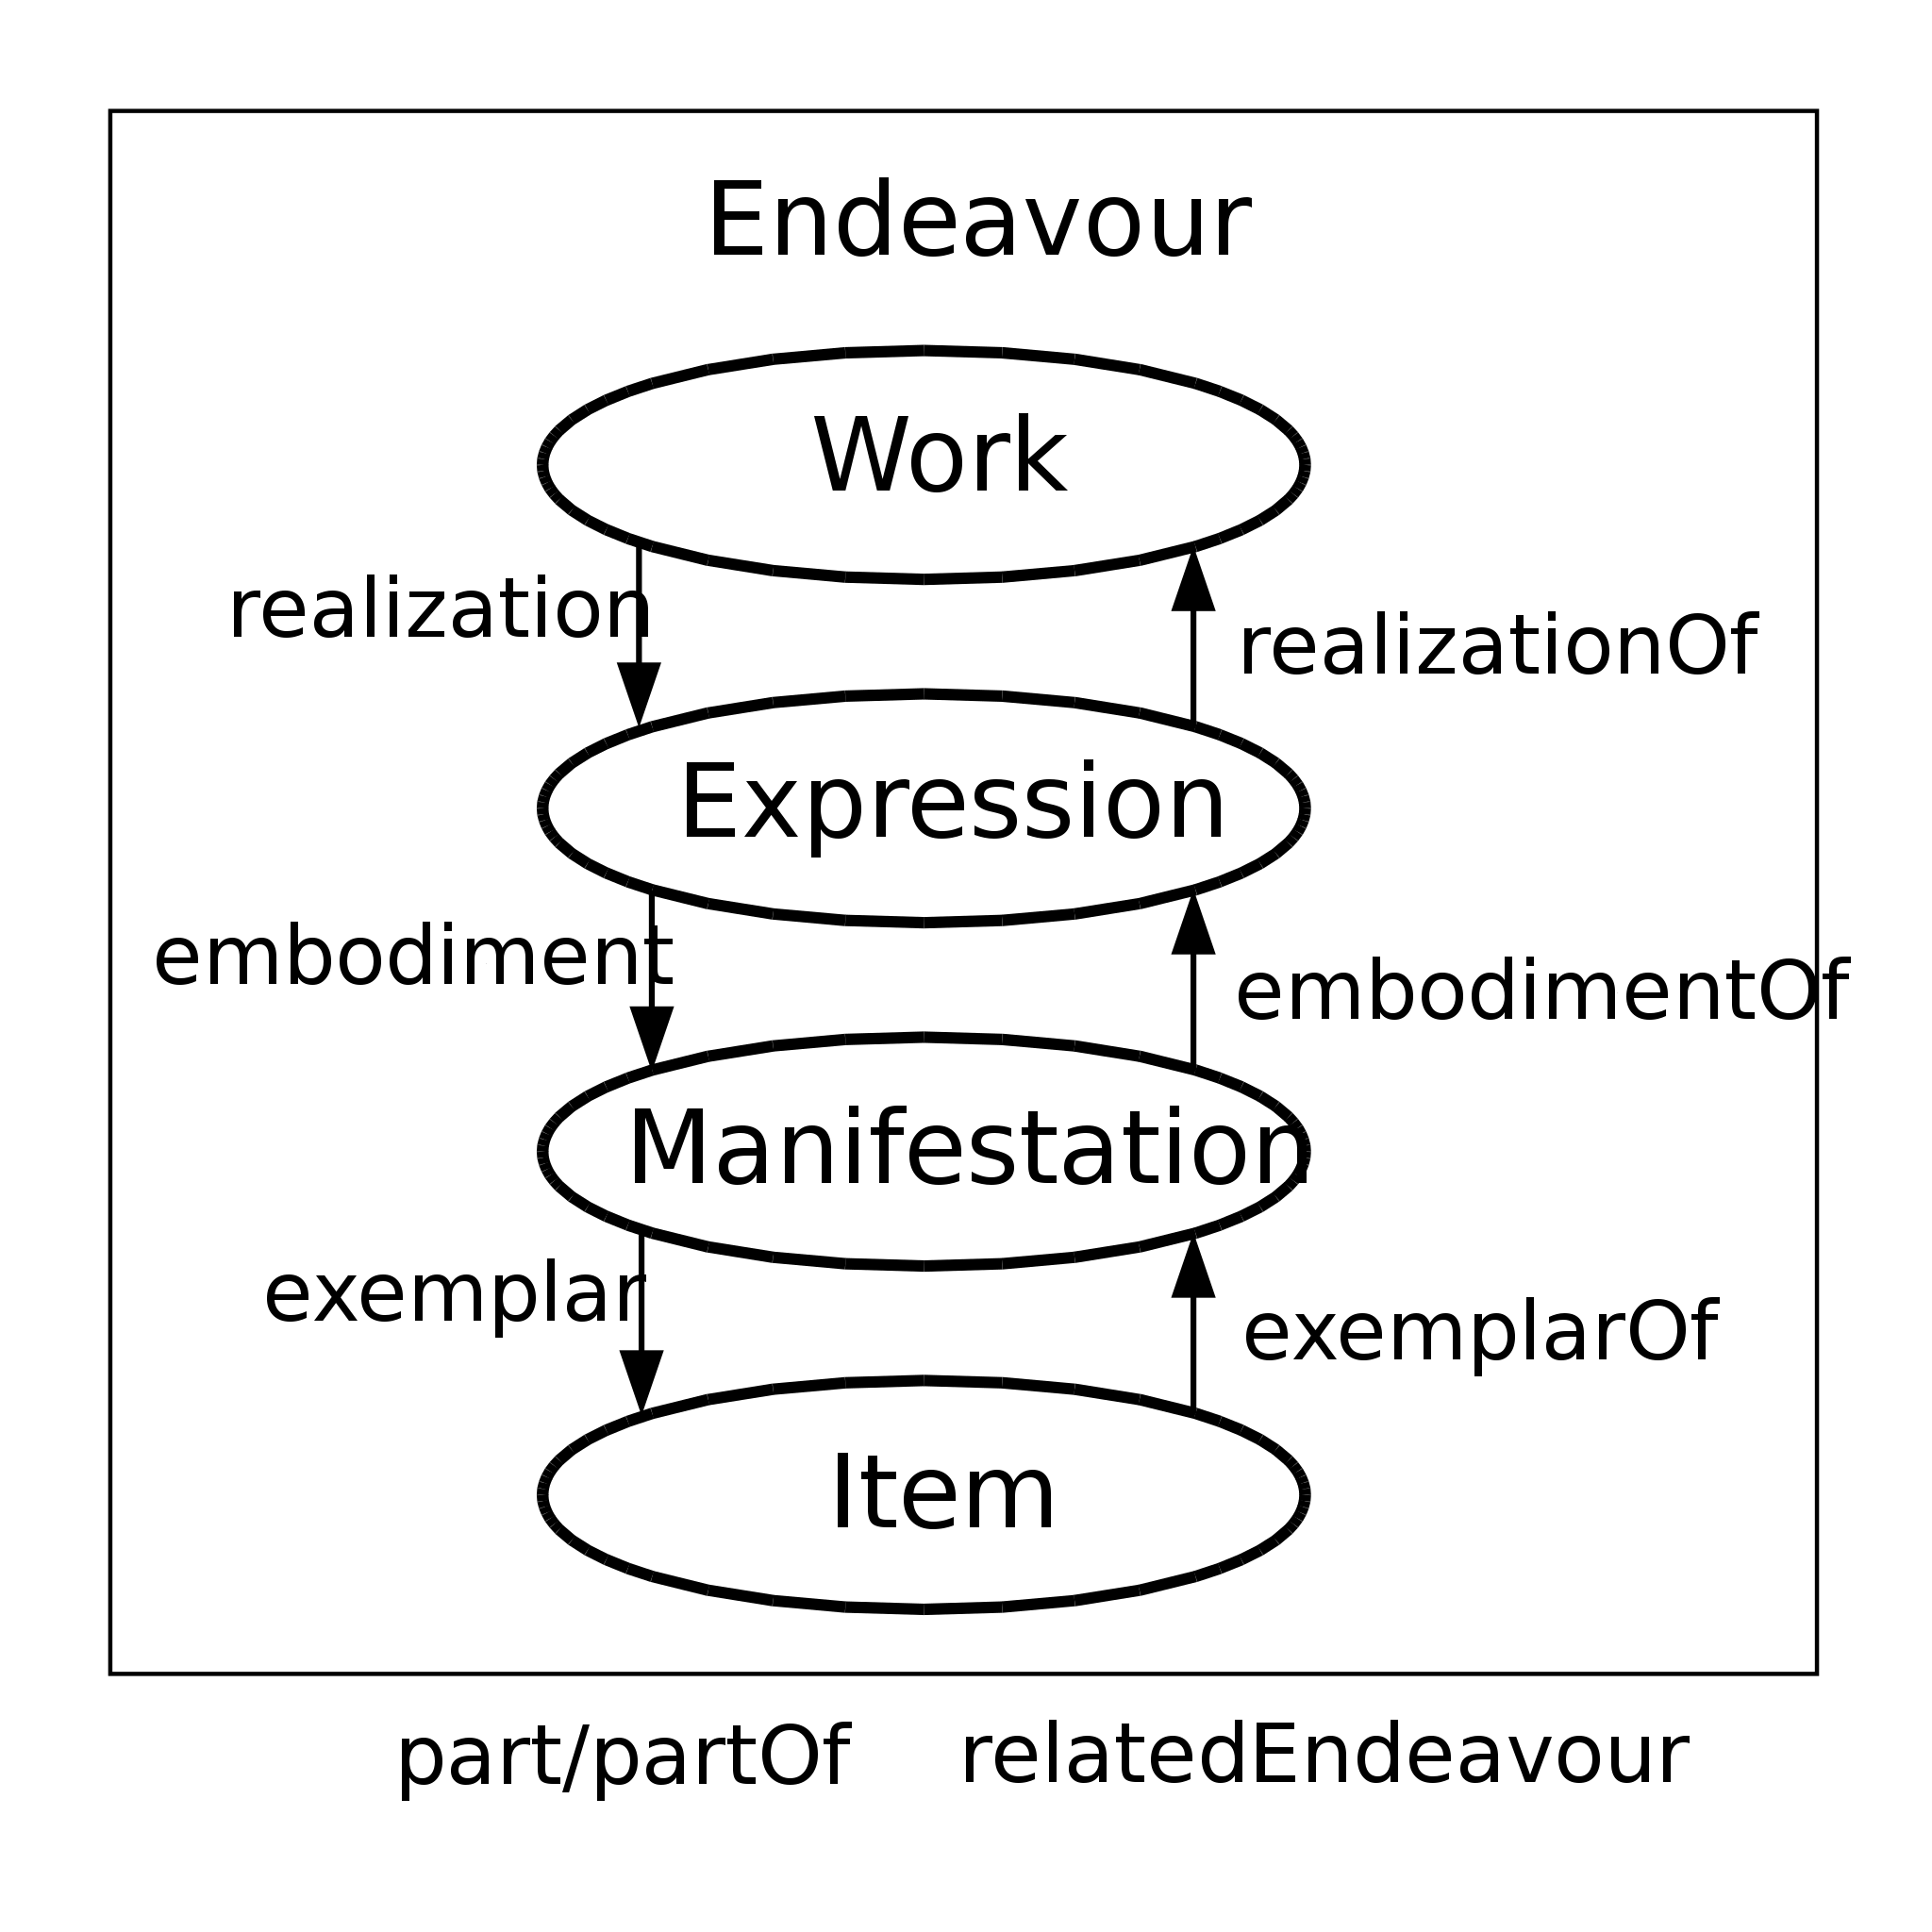
\includegraphics[height=60mm]{img/FRBR_Group1.png}
%  \qquad
%  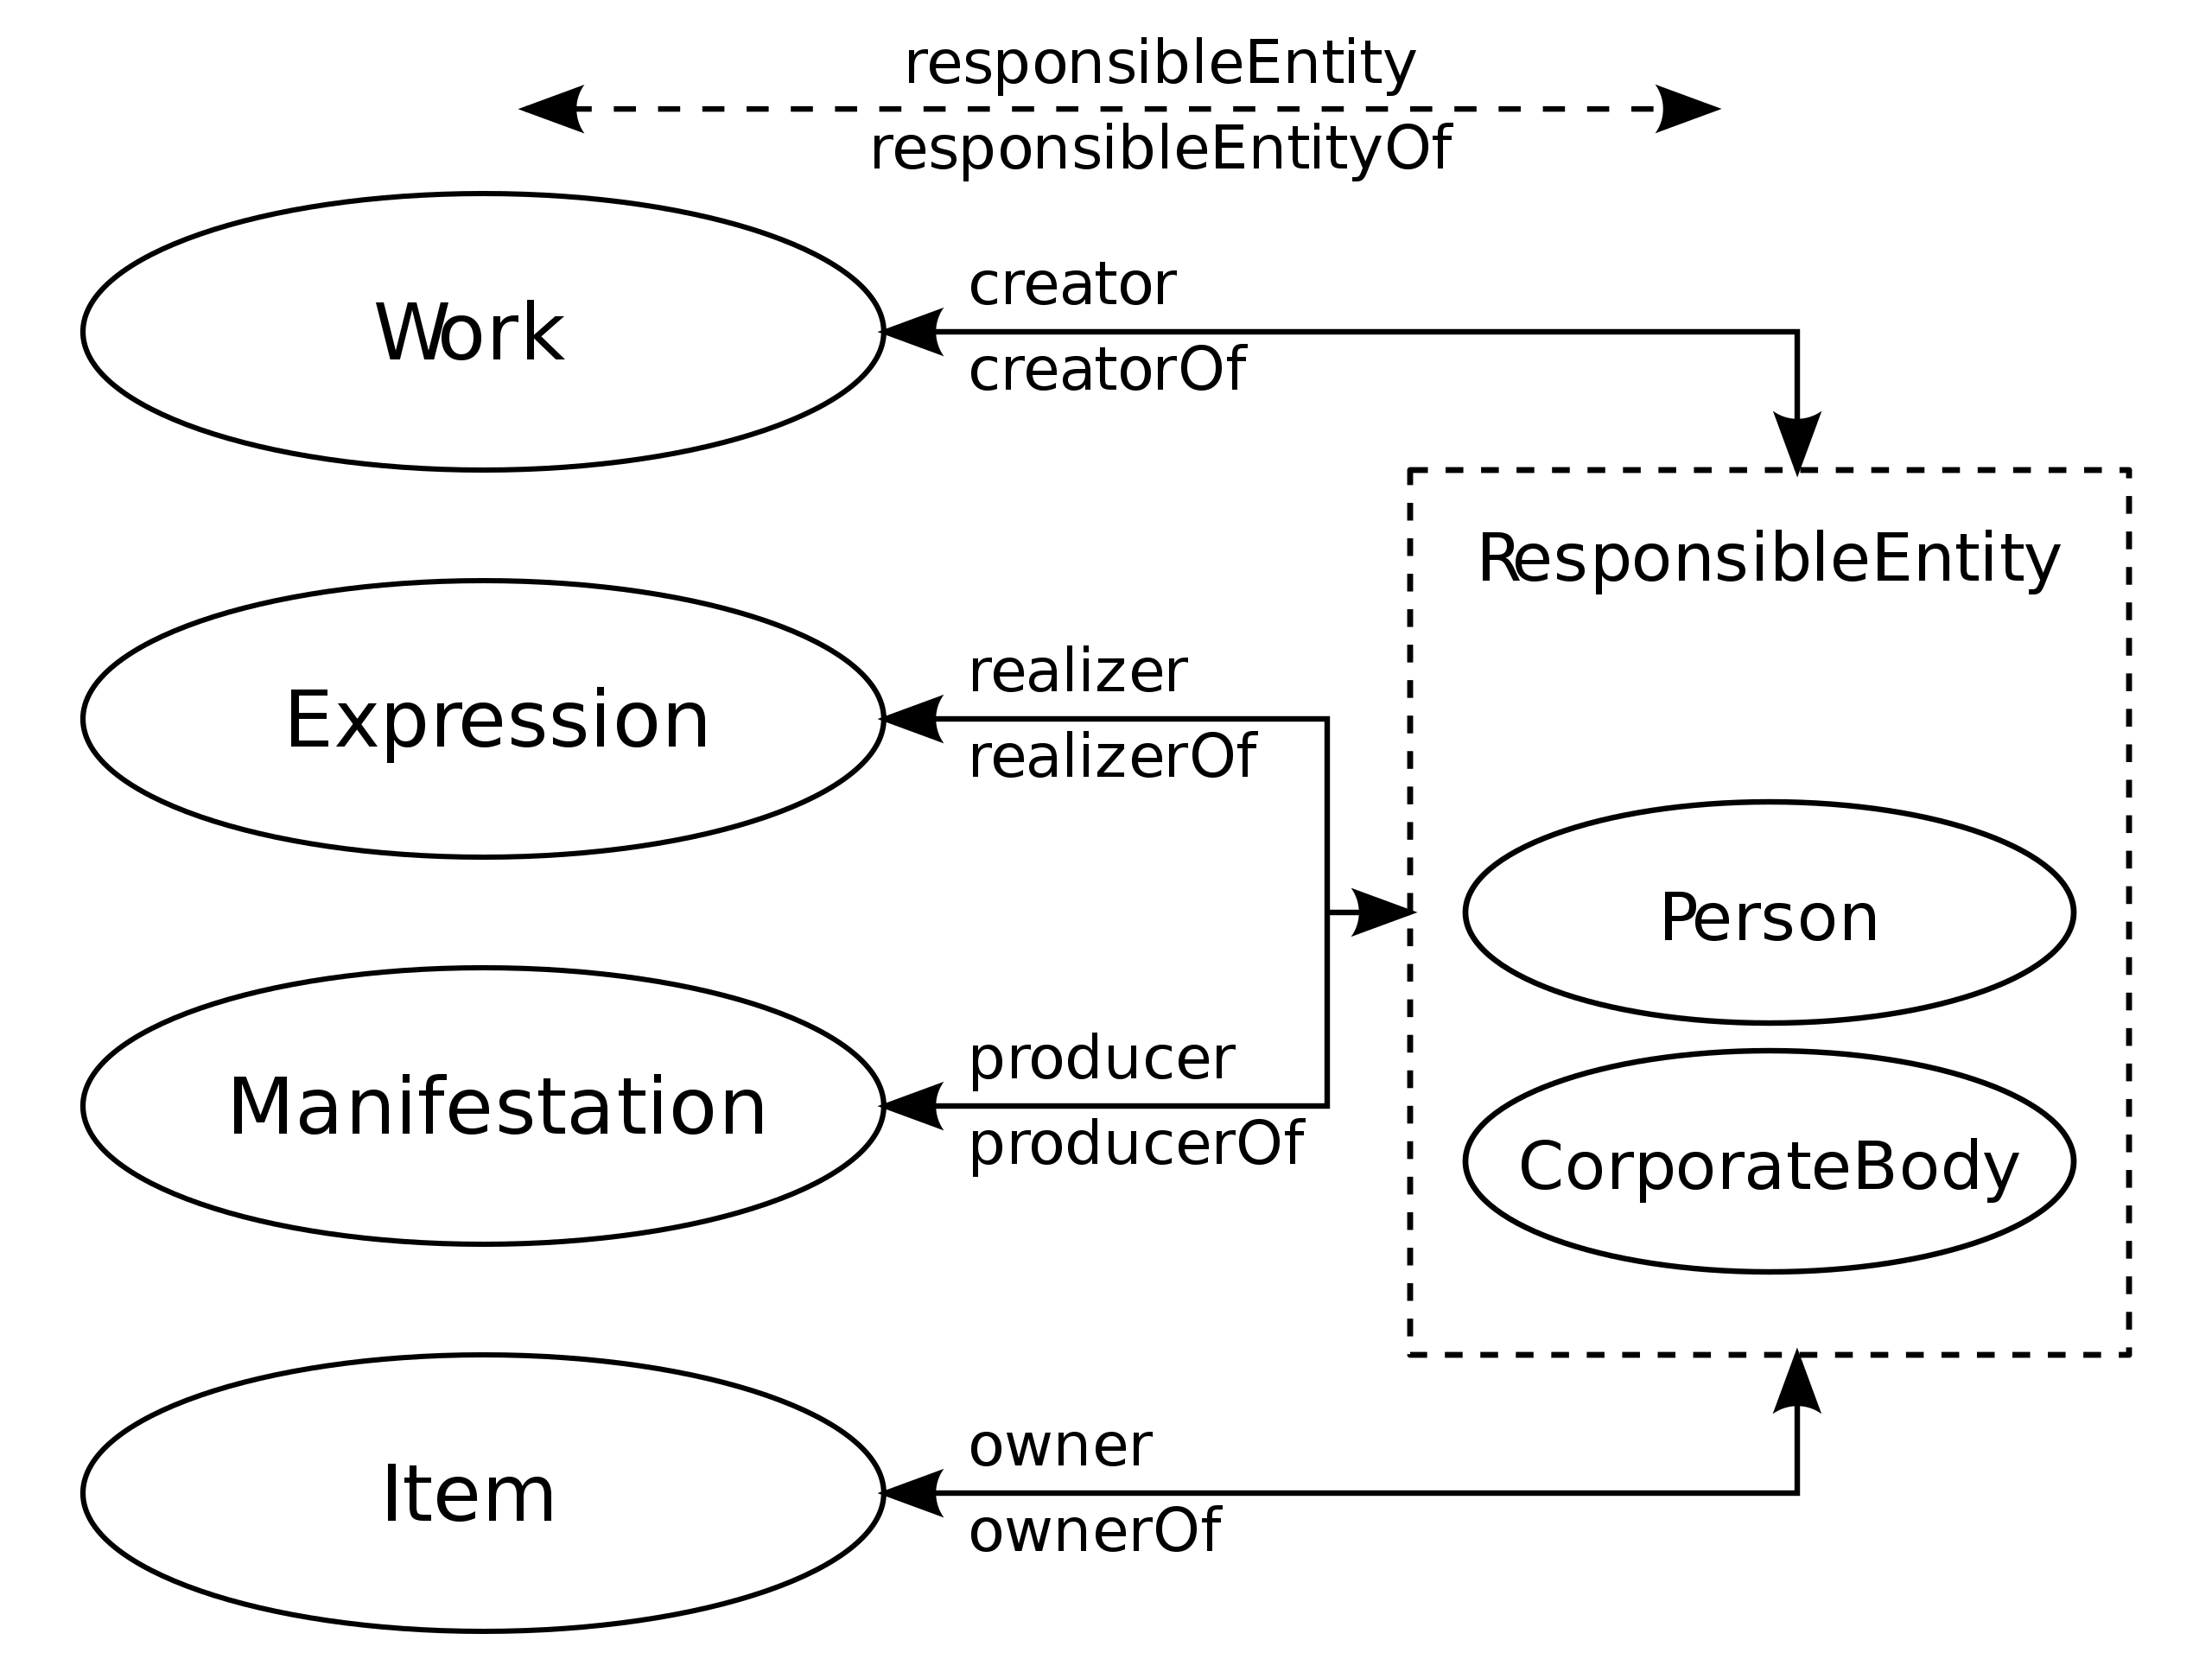
\includegraphics[height=60mm]{img/FRBR_Group2.png}
%  
%  \todo[defer,inline]{Make better picture? (see draft)}
%  
%  \caption[Basic FRBR entities and relations of Group~1 and Group~2]{%
%    \parbox[t]{.85\linewidth}{%
%      Basic \gls{FRBR} entities and relations of Group~1 (left) and Group~2 (right)
%      \par
%      \begin{footnotesize}
%        \href{https://commons.wikimedia.org/wiki/File:FRBR-Group-1-entities-and-basic-relations.svg}{\enquote{Basic Group 1 entities and relations of the FRBR model (RDF version)}} and
%        \href{https://commons.wikimedia.org/wiki/File:FRBR-Group-2-entities-and-relations.svg}{\enquote{Basic Group 2 entities and relations of the FRBR model (RDF version)}}
%        by \href{https://commons.wikimedia.org/wiki/User:JakobVoss}{Jakob Voss} are licenced under \href{https://creativecommons.org/licenses/by-sa/4.0/}{CC BY-SA 4.0}.
%        \par
%      \end{footnotesize}
%    }%
%  }
%%  \label{fig:FRBR}
%\end{figure}
%
\newlength{\manif}\settowidth{\manif}{\fns Manifestation}%
\newlength{\respe}\settowidth{\respe}{\fns ResponsibleEntity}%
\begin{figure}[ht]
  \centering
  \begin{tikzpicture}[
    >=Latex,
    every node/.style={on grid,rectangle,rounded corners=1mm,draw=black,fill=lightgreen,thick,inner sep=1.5mm},
    every edge/.style={draw=black,thick}
  ]
    % the 4 Group-1 entities
    \node                       (Work) {\fns\mystrut\tikzpb[\hspace*{\fill}]{\manif}{\term{Work}}};
    \node [below=12mm of Work]  (Expr) {\fns\mystrut\tikzpb[\hspace*{\fill}]{\manif}{\term{Expression}}};
    \node [below=12mm of Expr]  (Mani) {\fns\mystrut\tikzpb[\hspace*{\fill}]{\manif}{\term{Manifestation}}};
    \node [below=12mm of Mani]  (Item) {\fns\mystrut\tikzpb[\hspace*{\fill}]{\manif}{\term{Item}}};
    
    % their superterm Endeavour
    \node [above=11mm of Work, draw=none,fill=none,inner sep=0mm] (Ende) {\fns\mystrut\tikzpb[\hspace*{\fill}]{\manif}{\term{Endeavour}}};

    % placeholders plus rectangle for Endeavour
    \node [above left =1mm and 1mm of Work.north west,draw=none,fill=none,inner sep=.2mm] (WorkL) {};
    \node [below right=0mm and 1mm of Item.south east,draw=none,fill=none,inner sep=.2mm] (ItemR) {};
    \node [fit={(Ende) (WorkL) (ItemR)},fill=none] (G1E) {};
    
    % super-relations of Group-1 relations
    \node [left =8mm of Ende.180,draw=none,fill=none,inner sep=0mm] () {\fns\tikztabtwo[r]{\term{relatedEndeavour,}}{\term{part}}};
    \node [right=8mm of Ende.0  ,draw=none,fill=none,inner sep=0mm] () {\fns\tikztabtwo[l]{\term{relatedEndeavour,}}{\term{partOf}}};
    
    % the 2 Group-2 relations
%    \node [right=98mm of Expr] (Pers) {\fns\mystrut\tikzpb[\hspace*{\fill}]{\respe}{\term{Person}}};
%    \node [below= 8mm of Pers] (Corp) {\fns\mystrut\tikzpb[\hspace*{\fill}]{\respe}{\term{CorporateBody}}};
    \node [right=98mm of Item] (Corp) {\fns\mystrut\tikzpb[\hspace*{\fill}]{\respe}{\term{CorporateBody}}};
    \node [above= 8mm of Corp] (Pers) {\fns\mystrut\tikzpb[\hspace*{\fill}]{\respe}{\term{Person}}};

    % their superterm ResponsibleEntity
    \node [right=98mm of Ende, draw=none,fill=none,inner sep=0mm] (Resp) {\fns\mystrut\tikzpb[\hspace*{\fill}]{\respe}{\term{ResponsibleEntity}}};

    % placeholders plus rectangle for ResponsibleEntity
    \node [above left =1mm and 0mm of Pers.north west,draw=none,fill=none,inner sep=.2mm] (PersL) {};
    \node [below right=0mm and 0mm of Corp.south east,draw=none,fill=none,inner sep=.2mm] (CorpR) {};
    \node [fit={(Resp) (PersL) (CorpR)},fill=none] (G2E) {};

    % super-relations of Group-2 relations
    \node [left=6mm of Resp.180,draw=none,fill=none,inner sep=0mm] () {\fns\tikztabtwo[r]{\term{responsibleEntity/}}{\term{responsibleEntityOf}}};
    
    % placeholders for separating line
    \node [above=2mm of $(G1E.north east)!0.50!(G2E.north west)$,draw=none,fill=none,inner sep=.2mm] (SepN) {};
    \node [below=5mm of $(G1E.south east)!0.50!(G2E.south west)$,draw=none,fill=none,inner sep=.2mm] (SepS) {};
    
    \begin{scope}[%
      every node/.style={draw=none,fill=none,inner sep=.2mm}
    ]
      % Labels for groups
      \node [above  left=0mm and 2mm of SepS] () {\small Group 1};
      \node [above right=0mm and 2mm of SepS] () {\small Group 2};
      
      \path[->]
        % the 3 main Group-1 relations
        (Work) edge[out=195,in=165,looseness=3] node[left=1mm] {\fns\mystrut\term{realization}} (Expr)
        (Expr) edge[out=195,in=165,looseness=3] node[left=1mm] {\fns\mystrut\term{embodiment}}  (Mani)
        (Mani) edge[out=195,in=165,looseness=3] node[left=1mm] {\fns\mystrut\term{exemplar}}    (Item)
        
        % and their inverses
        (Expr) edge[out=15,in=345,looseness=3] node[right=1mm] {\fns\mystrut\term{realizationOf}} (Work)
        (Mani) edge[out=15,in=345,looseness=3] node[right=1mm] {\fns\mystrut\term{embodimentOf}}  (Expr)
        (Item) edge[out=15,in=345,looseness=3] node[right=1mm] {\fns\mystrut\term{exemplarOf}}    (Mani)
        
        % Group-2 relations
%        (Work) edge[out=5,in=150]  node[pos=.98,above left=1mm and 1mm,sloped] {\fns\mystrut\term{creator}}   (G2E)
%        (G2E)  edge[out=160,in=-5] node[pos=.02,below left=1mm and 1mm,sloped] {\fns\mystrut\term{creatorOf}} (Work)
        (Work.4)   edge node[pos=.98,above left=.2mm and 1mm] {\fns\mystrut\term{creator}}  ($(G2E.north west)!(Work.4)!(G2E.south west)$)
        (Expr.4)   edge node[pos=.98,above left=.2mm and 1mm] {\fns\mystrut\term{realizer}} ($(G2E.north west)!(Expr.4)!(G2E.south west)$)
        (Mani.4)   edge node[pos=.98,above left=.2mm and 1mm] {\fns\mystrut\term{producer}} ($(G2E.north west)!(Mani.4)!(G2E.south west)$)
        (Item.4)   edge node[pos=.98,above left=.2mm and 1mm] {\fns\mystrut\term{owner}}    ($(G2E.north west)!(Item.4)!(G2E.south west)$)

        % and their inverses
        ($(G2E.north west)!(Work.356)!(G2E.south west)$) edge node[pos=.02,below left=.2mm and 1mm] {\fns\mystrut\term{creatorOf}}  (Work.356)
        ($(G2E.north west)!(Expr.356)!(G2E.south west)$) edge node[pos=.02,below left=.2mm and 1mm] {\fns\mystrut\term{realizerOf}} (Expr.356)
        ($(G2E.north west)!(Mani.356)!(G2E.south west)$) edge node[pos=.02,below left=.2mm and 1mm] {\fns\mystrut\term{producerOf}} (Mani.356)
        ($(G2E.north west)!(Item.356)!(G2E.south west)$) edge node[pos=.02,below left=.2mm and 1mm] {\fns\mystrut\term{ownerOf}}    (Item.356)
      ;
    \end{scope}
    
    % draw separating line
    \path[-,dash pattern={on 6pt off 3pt}] (SepN) edge (SepS);
%        
  \end{tikzpicture}
  
%  \caption[Basic FRBR entities and relations of Group~1 and Group~2]{%
%    \parbox[t]{.85\linewidth}{%
%      Basic \gls{FRBR} entities and relations of Group~1 (left) and Group~2 (right)%
%    }%
%  }
  \caption[FRBR entities and basic relations of Groups~1 and~2]{\gls{FRBR} entities and basic relations of Groups~1 and~2 \autocite[following][]{FRBRpic1,FRBRpic2}}
  \label{fig:FRBR}
\end{figure}

Beside FRBR, the \gls{IFLA} developed
a conceptual entity-relationship model for authority data,
the \gls{FRAD},
as well as a continuation of FRBR,
the \gls{FRSAD}.

FRBR serves as a basic principle of RDA, which we discuss next.

% .............
\paragraph{RDA}

\gls{RDA} is a standard for the cataloguing of publications
in cultural heritage institutions, and particularly in libraries.
RDA is implemented and used in the library systems of several countries, including
the US, the UK, Canada, Australia, and the German-speaking countries
\autocite{WikiDE_RDA}.

RDA and the application guidelines for the German-speaking area
stipulate a special practice for recording FRBR Group-1 entities and relating 
them to each other: Bibliographic records (\enquote{Titel\-daten\-sätze})
have a bibliographic level for describing a manifestation
and an exemplar level for describing the related exemplars. The description of works and expressions
is considered part of the description of a manifestation and thus recorded at the bibliographic level.
However, it is possible to create and link an authority record for a work or expression
containing the relevant description. In that case, the source of the information can be recorded as well
\autocite[cf.][§5.1]{Wiesenmueller2015}.

For our approach, this observation means that catalogues of German libraries
do not use a uniform way of linking, e.g., a work $X$ with its manifestations.
In particular, if there is no authority record for $X$,
then $X$ is represented in the data of its manifestations only implicitly 
(and possibly ambiguously).


% -----------------------------------------------------------------
\section{Data Formats and Communication Protocols}
\label{sec:data_models}

In order to identify data sources in the following section,
we first need to describe relevant standards and formats for the description
and communication of (bibliographic) data.
The following discussion 
is based on~\citeauthor{Hider2008}'s overview \autocite*[§10]{Hider2008},
unless indicated otherwise.

% - - - - - - - - - - - - - - - - - - - - - - - - - - - - - - - - -
\subsection{Markup Languages}
\label{subsec:markup}

We briefly describe markup languages, which are repeatedly used in the technologies
described in the following subsections.
Markup languages are machine-readable languages used for the structuring and formatting of files.

% .................
\paragraph{HTML}
The most prominent example is the \gls{HTML}, the core language of the \gls{WWW}.
The markup features of HTML are also used to identify and describe certain elements of digital objects.
In particular, HTML provides for meta tags, i.e., labels for metadata.
One of the restrictions of HTML is its fixed set of labels, whose meanings cannot be changed.
Further standards were developed to overcome this restriction,
such as SGML and XML.

% .................
\paragraph{XML}
\glsreset{XML}%
The \gls{XML} is both a file format and markup language for the storage and transmission of arbitrary data;
it allows for a hierarchical structuring of data in a text file format that is readable by both humans and machines
\autocite{WikiXML}.
XML is the basis for many modern web developments.
Most metadata schemas have standard expressions in XML, as we will see below.

% - - - - - - - - - - - - - - - - - - - - - - - - - - - - - - - - -
\subsection{Data Communication Protocols}
\label{subsec:data_comm_prot}

% .............
\paragraph{Z39.50}

\glsreset{Z39.50}
is a protocol for data communication between bibliographic databases.
\glsunset{ISO}%
\glsunset{ANSI}%
\glsunset{NISO}%
It is an \gls{ISO} standard as well as an \gls{ANSI}/\gls{NISO} standard.
\glsunset{Z39.50}%
Z39.50 is a set of rules developed specifically
for translating search and retrieval commands between databases such as OPACs.
Using Z39.50, it is possible to issue commands specific to a local database
and obtain results from a remote database that might use a different command set.
This protocol can be implemented over the internet and similar networks.
Z39.50 is widely used in the library domain for providing access to catalogues,
for example, by the \gls{LoC}. Still, it is not fully implemented by all library systems,
and not all libraries use the most recent version. It is also not very widely spread
outside the library community.

% .............
\paragraph{SRU}

\gls{SRU} is a successor of \gls{Z39.50} and an \gls{LoC} standard.
It has the same function, which is the standardisation of search and retrieval
across online databases. 
SRU is based on \gls{HTTP}, \gls{XML}, and the \gls{CQL}, 
a standard syntax for representing queries to information retrieval systems.
Thanks to this technology, SRU is more dynamic than \gls{Z39.50}
and less restricted to the library domain.

% .............
\paragraph{OAI-PMH}

The \gls{OAI} is a project devoted to interoperability standards in information agencies
in general, including libraries.
The \gls{OAI-PMH} is a standard developed by the OAI
and is widely used in the library domain, albeit not as widely as \gls{Z39.50}.

% - - - - - - - - - - - - - - - - - - - - - - - - - - - - - - - - -
\subsection{Data Description Schemata}
\label{subsec:data_descr_schemata}

% .............
\paragraph{MARC}

\glsreset{MARC}
\gls{MARC} \enquote{is the main data communication standard in use in libraries today}
\autocite[p.198]{Hider2008}. It is a family of formats for the \emph{exchange} of bibliographic
and further data between library systems, which is being extensively used by libraries around the world. 
MARC was developed by the \gls{LoC} in 1969
and has been updated several times.
The MARC family comprises more than 20 dialects that have been developed as an official standard
in several countries.
Those are very similar to each other and provide very detailed record structures for cataloguing of bibliographic data.
They all adhere to an international \gls{ISO} standard.
The development of MARC pursued the goals of labour and cost reduction,
and of standardising the cataloguing process
as well as data communication and transfer.
MARC \enquote{allows flexibility in library information systems} \autocite[p.201]{Hider2008}
by providing an easy way of data exchange and allowing for better resource discovery (among others, in comprehensive union catalogues).

MARC~21, was developed in 1999 and is \enquote{the major version of MARC in use internationally} \autocite[p.205]{Hider2008}.
It consists of five formats for specific kinds of data.
Two of these are for bibliographic data and authorities data, respectively.

MARC has been criticised for its inflexible structure, the fragmentation into several dialects,
and the restricted compatibility with current computer technologies, among other things.
\textcite[p.212]{Hider2008} give more details and further references.
There have been several attempts to redeem some of these disadvantages,
among them the development of new standards such as MODS (see below)
and of \gls{XML} schemas based on MARC~21 such as MARCXML and Turbomarc.

The problem of the proliferation of standard was not restricted to the
variety of MARC dialects but also occurred within non-MARC formats.
Attempts to solve this problem have been made via
translation and unification. One tool for unification is Dublin Core (DC); see below.

Until recently, MARC~21 had separate data fields for the recording of provenance marks, owners,
and further information belonging to a provenance. As a consequence,
in data obtained via MARC~21, the important connection between provenance marks, owners,
and further information is not available.
For this reason, the MARC Steering Group approved, in May 2023, a proposal
%by the D-A-CH Working Group on Provenance, Task Group on MARC, in cooperation with the German National Library and the Committee on Data Formats
for introducing a new data field for
\enquote{Ownership and Custodial History in Structured Form} \autocite{MARC361proposal}.
This data field allows the structured recording of provenance information
by providing subfields for all the constituents of the same provenance.
However, it is realistic to assume that this new field
will be implemented in the relevant systems with some delay.

% .............
\paragraph{MAB}

The \gls{MAB}, translating as \enquote{machine data exchange format for libraries},
is a legacy bibliographic data format that has been developed solely for the purpose of data exchange
by the \gls{DNB}.
Although \textcite[p.204]{Hider2008} classify it as a dialect of \gls{MARC},
it is in fact conceptually different from \gls{MARC},
assigning exactly one bibliographic element to each data field
and allowing a more flexible ordering of elements \autocite{WikiMAB}.
In 2013, the \gls{DNB} completely abandoned the delivery of its bibliographic and authority data in MAB
in favour of \gls{MARC}~21 \autocite{MAB}.

% .............
\paragraph{MODS}

The \gls{MODS} is a standard developed by the \gls{LoC}
in order to overcome the problems with \gls{MARC} mentioned above.
MODS is based on \gls{XML} and a subset of MARC fields;
it can thus be used alongside MARC and as a \enquote{switching format
between MARC and non-MARC schemas} \autocite[p.219]{Hider2008}.
The LoC also maintains an analogous standard for authority data,
the \gls{MADS}.

% .............
\paragraph{DC}

\gls{DC} is an international standard consisting of 15 essential metadata terms
for describing digital or physical resources.
It was formulated by the \gls{DCMI}, a project of the US-American non-profit organisation
ASIS\&T, for the purpose of locating information resources on the \gls{WWW}.
The 15 core elements are tailored towards the \enquote{primary metadata needs} across domains
\autocite[p.215]{Hider2008}, thus making it a flexible data model.
Applications of \gls{DC} include resource description,
the combination of metadata vocabularies from different standards,
and the provision of interoperability in the linked data context.
\gls{DC} is extended by the \emph{DCMI Metadata Terms}.

%Sources of this summary are \textcite[§§1, 10]{Hider2008},
%and \citeauthor{WikiDC}~\autocite{WikiDC}.

% .............
\paragraph{RDF}

We have already introduced \gls{RDF} in Section~\ref{sec:linked_data+integration}.
In the context of the following description of data sources,
RDF is a very flexible data schema and the core technology for providing metadata as linked data.

% .............
\paragraph{BIBFRAME}

The \gls{BIBFRAME} is a data model for bibliographic description,
which was designed to replace the \gls{MARC} standards and use linked data principles
to improve access to bibliographic metadata within and outside the library domain \autocite{WikiBIBFRAME}.
The most recent version 2.0 was released by the \gls{LoC} in 2016 \autocite{BIBFRAME}.
So far, only a handful of libraries are using BIBFRAME,
most of them in test mode \autocite{WikiBIBFRAME}.

% -----------------------------------------------------------------
\section{Data Sources}
\label{sec:data_sources}

In this section, we collect and present information on data sources
that provide metadata on objects, individuals, concept membership, and relationships
(in short: \emph{terms})
relevant for provenance research.
Given the example queries discussed in Sections~\ref{sec:background}
and~\ref{sec:example_queries},
relevant terms include
the FRBR entities and relations (see Section~\ref{sec:bib_standards}),
ownership, as well as professional, familial, and social relationships.
We first give an overview of eligible data sources (Subsection~\ref{subsec:collection_data_sources})
and then select a few particularly relevant ones, for which we provide a detailed analysis
(Subsection~\ref{subsec:analysis_data_sources}).
The choice of the latter was motivated by the insights from the \gls{SoNAR} project (see Section~\ref{sec:HNA+SoNAR})
and Hakelberg's \autocite*[§4]{Hakelberg2016} overview of the state of provenance indexing with authority data
in the German-speaking area. This analysis will have to be extended
whenever the model and method that we are going to develop in the following chapters
is implemented in a retrieval system in future work.

% - - - - - - - - - - - - - - - - - - - - - - - -
\subsection{Collection of Data Sources}
\label{subsec:collection_data_sources}

We have identified four categories of relevant data sources:
library catalogues, special databases for provenance research, authority files, and knowledge bases.
We next describe, for each of these categories, the relevant information that is
contained in the respective data sources, and we list examples.

% .............
\paragraph{Library Catalogues}
%
%Library catalogues 
Catalogues contain the information relevant for provenance research, such as
%
\begin{itemize}
  \item
    bibliographic entities (works, expressions, manifestations, items);
  \item
    relations between these entities (e.g., \term{isManifestationOf});
  \item
    attributes for these entities (e.g., year of publication);
  \item
    people and corporate bodies and relations such as authorship;
  \item
    provenance entries (including, e.g., owners, the ownership relation, and further attributes such as the year of ownership);
  \item
    (implicitly) the current ownership;
  \item
    (ideally) references to entries in authority files for all these types of entities.
\end{itemize}
%
Examples of relevant library catalogues include
%
\begin{itemize}
  \item
    catalogues of national libraries, which often aim at collecting literature exhaustively
    and which are most likely to make metadata available in interoperable formats,
    in particular: \\
    \mybold{the catalogues of \gls{DNB}, \gls{LoC}, and the British Library} \autocite{DNBCatalogue,LoCcatalogue,BLcatalogue};
  \item
    meta-catalogues that enable a federated search in many catalogues,
    in particular: \\
    \glsunset{KVK}%
    \mybold{WorldCat} and the \mybold{\glsentrylong{KVK} (\gls{KVK})} \autocite{WorldCat,KVK};
  \item
    union catalogues of library networks, which combine the holdings of the participating libraries,
    in particular, the German union catalogues: \\
    \glsunset{B3KAT}
    \glsunset{hbz}%
    \glsunset{hebis}%
    \mybold{\gls{K10plus}, \gls{B3KAT},}
    the \mybold{union catalogues of \gls{hbz} and \gls{hebis}} \autocite{K10plus,B3KAT,hbz,hebis};
  \item
    catalogues and local systems of single libraries, if not covered by any of the above;
  \item
    special catalogues, e.g., those used for historical research in the \gls{SoNAR} project, %\todo{explain; relate to SoNAR or loot research}
    in particular: \\
    \mybold{\gls{ZDB}, \gls{KPE}, \gls{ZEFYS}, ExilePress} \autocite{ZDB,KPE,ZEFYS,ExilePress}.
\end{itemize}

Clearly, the integration of catalogues of the first three groups is preferable to the integration of catalogues of single libraries
because it would allow for an interaction with as few systems as possible while giving access to a large
combination of holdings. However, sometimes relevant information is recorded only in local library systems,
e.g., provenance entries in some of the \gls{SWB} libraries; see the description of \gls{K10plus} below.
In these cases, it is unavoidable to include these local systems.

% .............
\paragraph{Authority Files}
%
Authority files
contain information relevant for provenance research, such as
%
\begin{itemize}
  \item
    entities such as persons, corporate bodies, places, works;
  \item
    relations such as social relations, family relations, professional relations;
  \item
    attributes for the entities such as their profession.
\end{itemize}
%
They are usually subject to a strict quality control.
Examples include the \mybold{\gls{GND}} \autocite{GND} in the German-speaking area (which has been used extensively in \gls{SoNAR}),
\glsunset{LCNAF}%
\glsunset{ISNI}%
\glsunset{VIAF}%
the North-American \mybold{\gls{LCNAF}} \autocite{LCNAF},
and the international projects \mybold{\gls{ISNI} and \gls{VIAF}} \autocite{ISNI,VIAF}.

% .............
\paragraph{Knowledge Bases}

According to the insights from the \gls{SoNAR} project,
(open) \glspl{KB} can be useful when trying to overcome the problem with missing or unbalanced data
in authority files such as the \gls{GND} (see Section~\ref{sec:HNA+SoNAR}).
\Glspl{KB} are usually edited independently of the library domain by a wider community of contributors,
and their quality cannot be expected to meet the standards of catalogues or authority files edited by library personnel.
A prominent example of an open, cross-domain \gls{KB} is \mybold{Wikidata} \autocite{Wikidata},
which has tentatively been used in the context of the \gls{SoNAR} project
and which we have already identified in Section~\ref{sec:background} as possible source of metadata
for complementing authority data.

% .............
\paragraph{Cultural Heritage Databases}

This category contains generic federated portals of cultural heritage items
as well as special databases created especially for the support of provenance research.
Examples for the first kind of databases are \mybold{Europeana} \autocite{Europeana} (see Section~\ref{sec:linked_data+integration})
and the \mybold{\gls{DDB}};
an example for the latter is \mybold{Proveana}---the research database of the German Lost Art Foundation \autocite{Proveana}.

% - - - - - - - - - - - - - - - - - - - - - - - -
\subsection{Analysis of Data Sources}
\label{subsec:analysis_data_sources}

%\todo[defer,inline]{DISCUSS HeBIS? 68.. fields, unstructured; provenance mark cannot be linked to owner in case of several provenance entries}

We now provide a review of four data sources from the previous list, namely
\gls{DNB}, \gls{K10plus}, \gls{GND}, and Wikidata.
%\gls{KVK}, \gls{ZDB}, \gls{KPE}, Proveana, Europeana.
%
%The main goal of this analysis is to provide an exemplary overview of the features and specifics
%of these data sources, and to inform the model that we will develop in the subsequent chapter.
%In order to fulfil this purpose, it is not necessary to review all data sources listed above
%exhaustively.
%
%\todo[inline]{adapt this list and provide another brief justification for the choice?}
%
For each data source, we collect the following information.
%
\begin{itemize}
  \item
    \emph{Scope:}~
    thematic focus; coverage; number of records; standards for cataloguing
  \item
    \emph{Technical infrastructure:}~
    data format; data model; interfaces; support for linked data
  \item
    \emph{Data quality (from the \gls{SoNAR} grant proposal \autocite[p.\,19ff.]{SchneiderKempf2018}),
    if applicable:}~
    use of persistent identifiers and \glspl{URI}; adherence to standards for, e.g., time and date specification
  \item
    \emph{Features useful in the context of \gls{SoNAR} (see our discussion in Section~\ref{subsec:insights_from_SoNAR}), if applicable:}~
    recording of temporal attributes or relations; recording of data provenance
  \item
    Further features specific to the respective data source, if applicable
\end{itemize}

% .............
\paragraph{DNB}

The following information is taken from the \gls{DNB}'s websites under the category \enquote{DNB Professional} \autocite{DNB_coll_mand,DNB_cataloguing,DNB_metadata}.

The DNB adheres to a legal collection mandate, according to which
the DNB collects \enquote{all texts, images and sound recordings published in Germany or in the German language, translated from German or relating to Germany that have been issued since 1913}  \autocite{DNB_coll_mand}. This includes all physical publications, and, since 2006, electronic publications made available via the internet. The mandate commits the DNB to a complete and unbiased collection that includes, among others, \enquote{printed works compiled or published between 1933 and 1945 by German-speaking emigrants} \autocite{DNB_coll_mand}.

The DNB catalogues its entire collection both descriptively and by subject, 
adhering to standards such as \gls{RDA}, using authority data, and including persistent identifiers such as ISBN, ISSN, URN, and DOI.
The cataloguing data feeds the German National Bibliography.

According to the 2021 annual report \autocite{DNB_Jahresbericht_2021},
the DNB's holdings comprise 43.7 million physical or digitally accessible units, 
which are represented by almost 26 million records in the German National Bibliography.

Metadata can be obtained from the DNB freely (under the CC0 1.0 licence) via the interfaces
\gls{SRU} and \gls{OAI-PMH}, which support \gls{XML} serialisations of the data formats
\gls{MARC}~21, \gls{RDF}, DNB Casual (an \gls{XML}-based \gls{DC} format), and \gls{MODS}.
Further data formats are available via an individual access
to the DNB's \emph{Data Shop}.
The DNB's Linked Data Service provides open access to its bibliographic and authority data
in \emph{RDF} under the same license. Instructions on how to interact with these interfaces
are given on the DNB's webpage on metadata services \autocite{DNB_metadata}.
The DNB website also reports on a project for the conversion of its data
into the \gls{BIBFRAME} format \autocite[cf.][]{DNBBIBFRAME}:
for title records, the DNB OPAC provides a download button for the BIBFRAME format.
The state of this project beyond 2014 is left unclear.

According to the detailed specifications on the \gls{MARC} format by the DNB
\autocite{DNB_MARC21,DNB_MARCXML}, the recording of dates and times, languages,
geographic area codes, and countries conforms to the respective \gls{ISO} standards.
Since 2015, the DNB has been using \gls{MARC} field 883
for recording the metadata provenance for a selection of data fields
\autocite{DNBwiki_MARC_883}.
Furthermore, the DNB's MARC~21 schema provides for the cataloguing of the following temporal data concerning
title (i.e., manifestation) records: production, publication, distribution, and manufacturing dates
(including reproductions and reissues); notes on dates and times;
chronological subject term (as full text); graduation year (for dissertations etc.).

% .............
\paragraph{K10plus}

\glsunset{GBV}%
\glsunset{SWB}%
\gls{K10plus} is the joint catalogue of the German library networks \gls{GBV} and \gls{SWB}.
Together, these two networks comprise more than 1400 national, regional,
academic, and public libraries \autocite{BSZGBV,GBV_VZG},
of which 838 participate in K10plus, according to the list of participating institutions
in the K10plus Wiki \autocite{K10plusWiki}. Thus, K10plus comprises the data from
the majority of German academic institutions \autocite[cf.][]{BSZ_K10plus}.

As of 31 December 2022, K10plus contains 80.8 million bibliographic records (\enquote{Titeldatensätze})
with 235.4 million ownership records \autocite{GBV_K10plus_Statistik}.
Cataloguing adheres to the same standards and guidelines as in the DNB,
including similar specifications for the recording of temporal data and the use of ISO standards for dates, times, etc.
In addition, the structured variants of provenance indexing used in \gls{GBV} and \gls{SWB}
(see below) enable the recording of ownership dates if available.

K10plus provides metadata freely (under the CC0 1.0 licence),
mainly via the interfaces \gls{Z39.50} and \gls{SRU}.
Those support the data formats \gls{MARC}~21, (including its XML variants),
PICA+ and PICA-XML (two provider-specific internal data formats loosely based on MARC~21),
as well as \gls{DC}, \gls{MODS}, and the legacy format \gls{MAB}2.
Detailed instructions on how to interact with these interfaces
are given in the K10plus Wiki \autocite{K10plusWiki}.
In addition, snapshots of K10plus data are provided
in \gls{MARC}-XML and as linked open data (\gls{RDF}-XML), as per the information
in the K10plus Wiki \autocite{K10plusWikiOD}.
However, there are currently no recent snapshots,
but it is planned to provide them regularly in the near future.%
\footnote{Personal communication with Jakob Voß, VZG (head office of the \gls{GBV}).}

K10plus uses the \gls{GND} as the central authority file for disambiguating
persons, corporate bodies, works, subject terms, 
and further entities (see below for more details on the GND.).
For this purpose, K10plus includes 
copies of all \gls{GND} records, which are synchronised via an \gls{OAI-PMH} interface
within minutes after modification \autocite[cf.][]{K10plusHandbuchNormdaten}.
K10plus furthermore uses authority data from the \gls{BK} and the \gls{RVK},
cf.\ the K10plus Wiki \autocite{K10plusWikiNormdaten}.

Concerning the state of provenance indexing in the library networks \gls{GBV} and \gls{SWB},
Hakelberg \autocite*[§4]{Hakelberg2016} reports the following:
The catalogue systems of \gls{GBV} and \gls{SWB}, which are united in K10plus,
support the recording and display
of provenance marks at the bibliographic as well as the exemplar level of a record.
However, the practice of provenance indexing differs greatly between the two networks.
Since 2014, GBV has been advising the recording at the bibliographic level,
in order to allow provenance research across libraries. The respective data field
is structured similarly to the new MARC~21 field 361 (see Subsection~\ref{subsec:data_descr_schemata})
and thus keeps all information on the same provenance linked together.
Furthermore, the names of owners are linked
to the local authority record that represents, and redirects to, the respective record in \gls{GND}.
The physical provenance marks are documented via chains of terms from
\gls{T-PRO} (see Section~\ref{sec:provenance_indexing}) [plus dates if available].
As of 2014,
this standard was being tested and successively introduced in the participating libraries.
Before 2014, provenance marks were documented in free text in a data field for
exemplar-specific comments at the exemplar level, using \gls{T-PRO} descriptors 
and referring to local authority records that were \emph{not} directly linked to \gls{GND} records.
In contrast, the \gls{SWB} libraries have been, and still are, using a dedicated data field
at the exemplar level to record provenance marks.
This field provides subfields for the structured recording of T-PRO terms [and dates].
However, most \gls{SWB} libraries have abandoned the creation of exemplar records altogether
and thus needed to resort to using isolated local systems for provenance indexing \autocite[cf.][]{Hakelberg2016}.
These systems should therefore be included in the data sources to be accessed by a comprehensive retrieval system
for provenance relationships.

In summary, provenance marks are recorded within K10plus in a heterogeneous
and incomplete way, and developers of a retrieval system that uses K10plus have to
be aware of this problem.

% .............
\paragraph{GND}

\glsreset{GND}%
The \gls{GND}, is operated by the \gls{DNB}
\enquote{in cooperation with many other libraries, libra[r]y networks and other cultural and academic institutions.
At present, the GND contains around 9 million authority records for persons, corporate bodies, congresses, geographic entities, specialised terms and works; these are supplemented, updated and used frequently} \autocite{DNB_cataloguing}. More detailed statistics can be found in the DNB's
2021 annual report \autocite[p.49]{DNB_Jahresbericht_2021}.
GND adheres to the same cataloguing standards and offers the same technical infrastructure
as the DNB catalogue; in particular, GND data is accessible under the CC0 1.0 license alongside national bibliographic data
via the same interfaces and data formats, including several RDF serialisations.

The DNB's MARC~21 schema \autocite{DNB_MARC21}
provides for the cataloguing of the following temporal data in authority records:
biographical data (persons), date of publication (works), dates of existence (conferences, corporations),
year of discovery, dates of activity (persons, corporations), years of effect of relationships
between entities of different kinds. Examples for temporal data of the latter kind include
the time interval during which a scholar was member of a university or during which a person was another person's student.

We have already learnt from the \gls{SoNAR} project (Section~\ref{sec:HNA+SoNAR}) 
that the data in the GND is incomplete for several reasons.
A further reason is certainly connected with the individualisation guidelines
in the DNB's guidelines for recording persons and families in the GND
\autocite[part EH-P-16]{GND_Erfassungshilfen}, which specify the additional information
that needs to be provided in order to disambiguate a person or family.
These guidelines define two groups of features that can be used to individualise
(i.e., disambiguate) a person, such as biographical data or relationships to other persons, among many others.
Depending on the level of the respective authority record
(which indicates the state and quality of the record), one or only a few of the many features
from these two groups have to be recorded.
Therefore, there is no guarantee that, for example, relationships to other people
or temporal data of the kind mentioned above is recorded.
In addition, relationships to other people are recorded in an unnormed way,
using one of four very generic codes (e.g., acquaintance, professional relationship, family relationship)
and specifying the exact kind of relationship in free text.
Similarly, professions may be recorded in free text or via a link to an authority record.


%\todo[inline]{add insights from SoNAR (§~\ref{sec:HNA+SoNAR}) and DHa (see below)}
%
%DHa's remarks on GND vocabulary and richness of GND data:
%%
%\begin{itemize}
%  \item
%    \emph{Individualisierungsregeln}: relationships to other people are given in order to uniquely
%    identify the current person; there is no obligation to record relationships
%    (and GND does not claim to be an encyclopedia)
%  \item
%    relations are not normed:
%    e.g., field \enquote{Funktionsbezeichnung}: \$4 code \enquote{Eigenschaft der Beziehung},
%    specified by \$v \enquote{Freitext}
%  \item
%    professions are recorded in 678 \$b \enquote{biographische Anmerkung(en)} --
%    historically in free text,
%    more recently via link to the GND authority data for the respective profession (i.e., more standardised)
%  \item
%    Tp1 datasets: field 65 (6J?) \enquote{GND Systematik: eingeschr. Tätigkeit} (?),
%    query level 1 datasets?
%  \item
%    $\leadsto$ \mybold{look/read all this up!}
%\end{itemize}
%
%\dots

% .............
\paragraph{Wikidata}

Wikidata \autocite{Wikidata} is \enquote{a free, collaborative, multilingual, secondary database, collecting structured data to provide support for Wikipedia, Wikimedia Commons, the other wikis of the Wikimedia movement, and to anyone in the world} \autocite{Wikidata_intro}. Hence, there is no thematic restriction
on the content of Wikidata.

The main unit of information in Wikidata is the \emph{item}. Items \enquote{are used to represent all the \emph{things} in human knowledge, including topics, concepts, and objects} \autocite{Wikidata_items}.
Currently, Wikidata contains more than 100 million items \autocite{Wikidata_data_access}.
This number is two orders of magnitudes higher than the number of articles in Wikipedia
because Wikidata stores structured information on \emph{all} Wikimedia projects,
including the large media file repository Wikimedia Commons \autocite[cf.][]{Wikidata_items}.
Data on each item is stored in \emph{statements}, which have the same \gls{SPO}
form as \gls{RDF}, in Wikidata terms: \emph{item--property--value}.
Statements can have annotations
\autocite[cf.][]{Wikidata_statements}. All items and properties have unique identifiers
consisting of a \term{Q} or \term{P}, respectively, followed by a sequence of digits.
These IDs are also part of the URL of the respective Wikidata page
and of the item's or property's URI.
For example, the item representing the 
Polish mathematician and astronomer Nicolaus Copernicus has the ID \term{Q619},
and the statements about this item are listed on the respective Wikidata page \autocite[cf.][]{Wikidata_Copernicus}.
The first statement in this list says that Copernicus is a human,
using the property \term{instance\_of} (\term{P31}) and the value \term{human}
(item \term{Q5}).

Data is recorded in Wikidata collaboratively,
i.e., \enquote{[d]ata is entered and maintained by Wikidata editors, who decide on the rules of content creation and management. Automated bots also enter data into Wikidata}
\autocite{Wikidata_intro}.
Values such as times and dates are recorded conforming to the respective \gls{ISO} standard.

The Wikidata page on data access \autocite{Wikidata_data_access} lists numerous ways to access data,
all under the free CC0 license.
For retrieving individual entries via URIs, there is a linked data interface.
For retrieving a relatively small set of entries that are not known in advance,
SPARQL queries can be posed against the Wikidata Query Service.
For retrieving larger sets of entries, Wikidata offers the Linked Data Fragments endpoint,
which requires computational power on the client side.
Furthermore, there are two APIs mostly for editing Wikidata,
as well as a recent changes stream and complete exports (dumps)
\autocite[cf.][]{Wikidata_data_access}.

Annotations of statements (see above) seem to be suitable for 
recording metadata provenance and temporal attributes of relationships.
It remains to investigate the use of annotations systematically
in order to determine the extent to which metadata provenance and temporal attributes
are recorded.

%\par\bigskip
%\todo[inline,defer]{If there is time left, then also describe: Proveana, ZDB, KPE, Europeana, WorldCat, KVK ::}
%
%\begin{itemize}
%  \item
%    \mybold{KVK} (\enquote{federated search}: shallower than in single catalogues,
%    but (sufficient) information on all copies!);
%    further catalogues?  
%\end{itemize}

%\todo{section on Data Integration and Further Techniques :: }
%% -----------------------------------------------------------------
%\section{Data Integration and Further Techniques}
%\label{sec:data_integration}
%
%\begin{itemize}
%  \item 
%    ETL (from grant proposal \gls{SoNAR}, p.~8, AP1-1)
%  \item
%    upper-level ontologies?
%  \item 
%    ontologies on research
%  \item
%    FRBRoo?
%  \item
%    \gls{RDF}, \gls{SPARQL}, N-Quads?
%\end{itemize}

% -----------------------------------------------------------------
\section{Conclusions}
\label{sec:implications_on_modelling}

We have collected 20 data sources and reviewed four of them in detail.
These four have in common that they provide their metadata as linked data (among other formats),
and the three bibliographic data sources adhere to the FRBR entity-relationship model.
From this commonality, we conclude that entities and relationships---%
in mathematical terms, constants and unary and binary relations---%
should play a central role in the model of queries, answers, and data sources
that we are going to develop next. This means that a graph-based type of model,
which also features in the \gls{SoNAR} project,
is suitable. In case relations of higher arity turn out to be required,
for example when representing the  provenance of an \gls{SPO} statement,
those can always be represented by several binary relations via reification
\autocite[cf.][p.339f.]{Doan2012}.

The choice of the reviewed data sources was motivated by the insights from
the \gls{SoNAR} project and Hakelberg's thesis \autocite{Hakelberg2016}.
For the abstract model to be developed next,
the specific choice of data sources is largely unimportant
because the model should be independent on the contents or specific data models of the sources.
The same holds for the general method for answering queries that we are going to develop based on our model.
However, future implementations of our method will have to take the specifics
of the data sources into account.
For this reason, it will be necessary to review additional data sources,
compare them quantitatively with respect to the extent and quality of their data,
and find structured ways for dealing with the problems concerning the data quality
reported above, such as the ambiguous links to works and expressions in RDA-based
catalogues, the heterogeneous and partly unstructured recording of provenance,
and the bias and incompleteness of the \gls{GND}.
The latter problem might be alleviated by using Wikidata
(sacrificing the strict quality control of the GND),
and promising candidates for alternative databases with extensive provenance information
are Proveana, the \gls{DDB}, and Europeana.%
\footnote{%
  Unfortunately, Proveana does not currently offer interfaces for automated data access,
  as communicated by Sabrina Werner, the Proveana project manager of the German Lost Art Foundation.
  For possible alternatives, Ms Werner referred to the \gls{DDB} and Europeana.%
}
